% FUSAO (26/10/2026): float copied unchanged from tables_C*.tex, tables_main.tex or tables_appendix.tex.
\begin{figure}[htbp]\centering
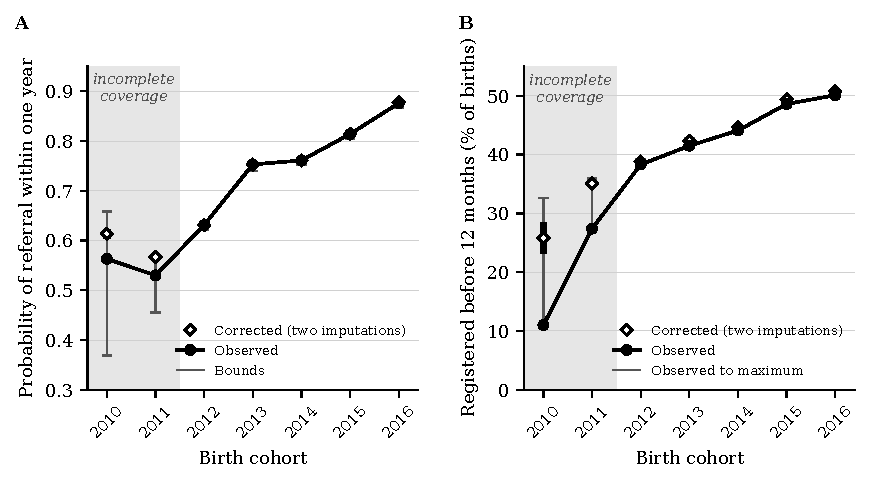
\includegraphics[width=0.95\textwidth]{V3_fig_level}
\caption{Observed and corrected levels by birth cohort for a service measure and a count}
\label{fig:level}
\tabnote{\emph{Sources:} SME childcare request record (applications dated 2010--2018, with referral dates through November 2019); SME enrolment records (EOL), entries through December 2018; SINASC live births. \emph{Sample:} applicants with eligible time in each birth cohort, plus the cohort's entrants with no request recorded before entry. Panel A shows referral within 365 days of the first application; Panel B shows children registered before 12 months as a percentage of live births. Circles are levels observed in the request record. Thick bars and diamonds show the corrected level as the range and midpoint of two imputations, defined in the note to Table~\ref{tab:level}. Thin lines show the bounds in Panel A and the range from the observed level to the maximum in Panel B. Shaded cohorts have applications partly in semesters of incomplete coverage. The figure is descriptive; Table~\ref{tab:level} reports the values for the 2010--2013 and 2016 cohorts.}
\par\smallskip\noindent\begin{minipage}{\linewidth}\footnotesize\raggedright Alt text: Two-panel chart organized by birth cohort from 2010 to 2016. Each panel displays observed estimates as circles and corrected estimates as diamonds with thick uncertainty bars. Thin lines indicate the corresponding bounds across cohorts.\end{minipage}
\end{figure}
